$\overrightarrow{A} - \overrightarrow{C}$

\begin{solution}\
\begin{center}
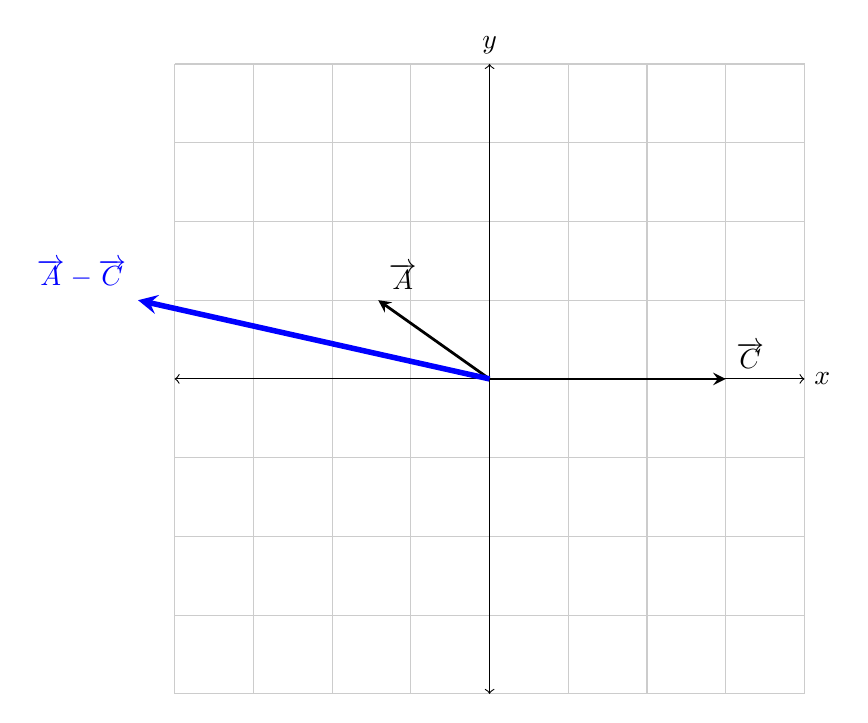
\begin{tikzpicture}
  \draw[thin,gray!40] (-4,-4) grid (4,4);
  \draw[<->] (-4,0)--(4,0) node[right]{$x$};
  \draw[<->] (0,-4)--(0,4) node[above]{$y$};
  \draw[line width=1pt,black,-stealth](0,0)--(-1.414,1) node[anchor=south west]{$\overrightarrow{A}$};
  \draw[line width=1pt,black,-stealth](0,0)--(3, 0) node[anchor=south west]{$\overrightarrow{C}$};
  \draw[line width=2pt,blue,-stealth](0,0)--(-4.464, 1) node[anchor=south east]{$\overrightarrow{A}-\overrightarrow{C}$};
\end{tikzpicture}
\end{center}
\end{solution}